% !TeX spellcheck = en_GB
\documentclass[DIV=12]{scrartcl}
\usepackage[utf8]{inputenc}

\usepackage[english,british]{babel}


\usepackage{graphicx}
\usepackage[style=american]{csquotes}
\usepackage{xspace}

\newcommand{\eg}{e.\,g.\@\xspace}

\author{Tobias Käfer\thanks{Karlsruhe Institute of Technology (KIT). \url{http://www.aifb.kit.edu/web/Tobias_K\%C3\%A4fer}}}
\title{Distributed COVID-19 Knowledge Graph Practical Assignment}

\usepackage[pdfborder={0 0 0}]{hyperref}

\begin{document}
\maketitle


\section*{Scenario}

Imagine you are running a courier service from a town in the Regierungsbezirke/NUTS-2 regions around the city of Karlsruhe: the regions of Karlsruhe and Darmstadt, or the very western part of Lower Franconia and the south-eastern part of Rhineland-Palatinate, see Figure~\ref{fig:karlsruhe-surroundings}.

\begin{figure}[h]
\centering
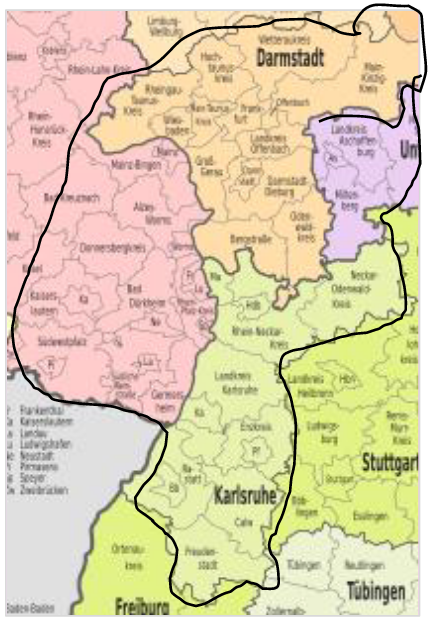
\includegraphics[width=0.4\textwidth]{karlsruhe-surroundings}
\caption{Karlsruhe and its surroundings. Based on {\tiny \url{https://de.wikipedia.org/wiki/Landkreis\#/media/Datei:Germany,_administrative_divisions_(+districts)_-_de_-_colored.svg}}.\label{fig:karlsruhe-surroundings}}
\end{figure}

For your route planning, you need to know which lockdown rules are currently valid in the regions of your customers, which we also assume to be in those regions.
As the lockdown rules have state-scope (Länder, NUTS-1), but the infection figures are published per region (Kreise, NUTS-3) we are facing an integration problem.

To assist the companies, we collaboratively build a data set in three phases:

\section{Create and Publish Data}

\begin{itemize}
\item Pick a town/municipality in those regions, \eg whose name starts with the first letter of your first name.
\item Invent a fictitious courier company, \eg \enquote{ACME Inc.}, which shall be located in this town
\item Write a Turtle file with 15-25 RDF triples describing the company:
\begin{itemize}
\item Some interesting properties to describe the company: name, post code, services offered, customers. The description of customers should have at least a post code.
\item Read the news about the NUTS-3 region (Kreis) of the company and add a n-ary relation with COVID-19 infections (daily total), timestamp, and postcode
\item Be creative and make up properties to describe the resources!
\item Per URI you mint, add at least one triple that uses \nolinkurl{rdf:type} or its short form \nolinkurl{a} as predicate, as it is good practice to say of what type a thing is.
\end{itemize}
\item Create a SoLiD Pod\footnote{Find some providers at \url{https://solidproject.org/users/get-a-pod}, or use your student's webspace} for the company
\item Update the SoLiD Pod by copying and adapting triples from the Turtle file
\item Hand in the URI of your fictitious company.
\end{itemize}


\section{Query Data and Lift Data to RDF}

\begin{itemize}
\item Lift the post-code-to-NUTS-mapping\footnote{\url{https://ec.europa.eu/eurostat/web/nuts/correspondence-tables/postcodes-and-nuts}} to RDF, \eg using tarql\footnote{\url{https://tarql.github.io/}}. Make the URIs for the NUTS codes start with \nolinkurl{http://data.europa.eu/nuts/code/}.
\item Add the lifted data to your SoLiD Pod.
\item Add to the data another n-ary relation with the current threshold for curfew in your state and the NUTS-1 code of your state
\item Find out the WikiData URI for the NUTS region of your company and double-check that there is population data for the NUTS region of your company in Wikidata.
\item Write a SPARQL query that finds out the infection numbers per 100\,000 inhabitants in the regions of your company's customers. Hints: You may want to\dots
\begin{itemize}
\item Have multiple \texttt{FROM} clauses for:
\begin{itemize}
\item The customer data from your SoLiD Pod
\item The NUTS-postcode mapping from your SoLiD Pod (may also be included in the previous RDF graph)
\item The URI of the region in Wikidata
\end{itemize}
\item Use \texttt{BIND} to calculate the division and assign the result to a variable.
\end{itemize}

\item Upload the SPARQL query to your Pod and hand in the URI of the query.
\end{itemize}


\section{Integrate Data and Follow Links}

\begin{itemize}
\item The supervisors provide you with URIs of companies in other students' data
\item Add \nolinkurl{foaf:based_near} links to your data that connect the your company to companies in adjacent NUTS-3 regions, thus building a list of local companies.
\item Add \nolinkurl{rdfs:subPropertyOf} links to your data that map the properties you defined in Phase 1 and 2 to:
\begin{itemize}
\item \nolinkurl{rdfs:label} for the name
\item \nolinkurl{vcard:postal-code} for the post code
\item \nolinkurl{swt:cvdinfections} for the infection number
\item \nolinkurl{swt:cvdcurfewthreshold} for the threshold
\end{itemize} 
\item Add \nolinkurl{rdfs:subClassOf} links to your data that map the classes you defined in Phase 1 and 2 to:
\begin{itemize}
\item \nolinkurl{foaf:Organization} for the class of all companies
\end{itemize}
\item Again, hand in the URI of your company.
\end{itemize} 


\section*{Putting it all together}

The supervisors can then:
\begin{itemize}
\item Seeded with the URIs of the companies from Phase 1, explore the graph by following \nolinkurl{foaf:based_near} links
\item Integrate the data using RDFS entailment
\item Build a SPARQL query that provides for each customer of a given company the current COVID-19 situation by:
\begin{itemize}
\item calculating the infection number per 100\,000 inhabitants for each NUTS-3 region
\item checking for each region (NUTS-3) whether the infection number per 100\,000 inhabitants is above the state's (NUTS-1) threshold\footnote{Hereby, use the mappings between NUTS levels as provided at \url{https://data.europa.eu/euodp/repository/ec/estat/nuts/nuts.rdf}.}
\end{itemize}
\item Alternatively, build a SPARQL query that outputs the result per NUTS-3 region in order to display them on a map\footnote{Hereby, use the SPARQL XML result format, which can be transformed using an XSLT transformation to the KML format. KML can be imported to many mapping applications including Google Earth, which allows for nice display of the results.}
\end{itemize}
These steps can be built on top of Linked Data-Fu\footnote{\url{http://linked-data-fu.github.io/}}.
Hereby, the calculations and \texttt{BIND} have to be turned into triples that make use of the CWM built-in functions vocabulary\footnote{\url{https://www.w3.org/2000/10/swap/doc/CwmBuiltins}}.

\section*{Acknowledgements}
Matthias Farnbauer-Schmidt provided helpful input on this exercise.

\clearpage
\appendix

\section*{Useful Tools}

There are online services and tools to install on your local machine, which may be handy to check your solutions.

\subsection*{Online Services}

\begin{itemize}
\item You can check whether your RDF is valid at \url{http://rdfshape.herokuapp.com/dataConversions}
\item You can find out what commonly used prefixes to build CURIES typically refer to at \url{http://prefix.cc/}
\end{itemize}

\subsection*{Command-line Tools rapper and roqet}

Using the \texttt{rapper} command, you can dereference a URI (or read from disk) and parse the received RDF:
\begin{verbatim}
rapper -i turtle <URI>
\end{verbatim}
Using the \texttt{roqet} command, you can execute a SPARQL query from a given URI (or from disk), which dereferences the URIs given in \texttt{FROM} clauses of SPARQL queries:
\begin{verbatim}
roqet <URI>
\end{verbatim}
The command-line tools \texttt{rapper} and \texttt{roqet} are available for different operating systems:

\subsubsection*{Installation on Linux}
You can install the tools on Debian-based Linux distributions (such as Ubuntu) using:
\begin{verbatim}
sudo apt-get install rasqal-utils raptor2-utils
\end{verbatim}


\subsubsection*{Installation on Windows}

On Windows, the easiest is probably you have access to a Linux server via \verb|ssh|.
There are more (not-so-easy) options:
\begin{itemize}
\item You install Ubuntu for Windows\footnote{\url{https://ubuntu.com/tutorials/ubuntu-on-windows}} and follow the instructions for Linux (untested).
\item You install the Cygwin subsystem and add the mentioned tools:
\begin{enumerate}
\item Follow the instructions at \url{https://www.cygwin.com/install.html}
\item Add the third-party repository \url{https://sourceware.org/cygwinports/}
\item Install the packages \verb|rasqal| and \verb|raptor2|
\end{enumerate}
\end{itemize}

\subsubsection*{Installation on MacOS}

Using HomeBrew\footnote{\url{https://brew.sh/}}, install the packages \verb|rasqal| and \verb|raptor| (untested).



\end{document}